\documentclass[11pt]{article}
\usepackage{amsgen,amsmath,amstext,amsbsy,amsopn,amssymb}
%\usepackage[dvips]{graphicx,color}
\usepackage{graphicx,color}
\usepackage{graphicx,color,bm}
\usepackage{epsfig}
\usepackage{enumerate}
\usepackage{ amsthm}
\usepackage{float}

%\setlength{\oddsidemargin}{0.1 in} \setlength{\evensidemargin}{-0.1
%in} \setlength{\topmargin}{-0.6 in} \setlength{\textwidth}{6.5 in}
%\setlength{\textheight}{8.5 in} \setlength{\headsep}{0.75 in}
%\setlength{\parindent}{0 in} \setlength{\parskip}{0.1 in}

\textwidth 6.3in \textheight 8.8in \topmargin -0.5truein
\oddsidemargin .15truein
\parskip .1in
\renewcommand{\baselinestretch}{1.53}  % double spaced


\newcommand{\homework}[6]{
	\pagestyle{myheadings}
	\thispagestyle{plain}
	\newpage
	\setcounter{page}{1}
	\noindent
	\begin{center}
		\framebox{
			\vbox{\vspace{2mm}
				\hbox to 6.28in { {\bf Math531:~Regression - I  \hfill} }
				\vspace{6mm}
				\hbox to 6.28in { {\Large \hfill #1 (#2)  \hfill} }
				\vspace{6mm}
				\hbox to 6.28in { {\it Instructor: #3 \hfill} }
				\hbox to 6.28in { {\it Office hours: #4  \hfill #6}}
				\vspace{2mm}}
		}
	\end{center}
	\markboth{#1}{#1}
	\vspace*{4mm}
}

% ----------------------- MATH -------------------------
\def\av{\boldsymbol a}
\def\bv{\boldsymbol b}
\def\cv{\boldsymbol c}
\def\dv{\boldsymbol d}
\def\ev{\boldsymbol e}
\def\fv{\boldsymbol f}
\def\gv{\boldsymbol g}
\def\hv{\boldsymbol h}
\def\iv{\boldsymbol i}
\def\gv{\boldsymbol j}
\def\kv{\boldsymbol k}
\def\lv{\boldsymbol l}
\def\mv{\boldsymbol m}
\def\nv{\boldsymbol n}
\def\ov{\boldsymbol o}
\def\pv{\boldsymbol p}
\def\qv{\boldsymbol q}
\def\rv{\boldsymbol r}
\def\sv{\boldsymbol s}
\def\tv{\boldsymbol t}
\def\uv{\boldsymbol u}
\def\vv{\boldsymbol v}
\def\wv{\boldsymbol w}
\def\xv{\boldsymbol x}
\def\yv{\boldsymbol y}
\def\zv{\boldsymbol z}
\def\Av{\boldsymbol A}
\def\Bv{\boldsymbol B}
\def\Cv{\boldsymbol C}
\def\Dv{\boldsymbol D}
\def\Ev{\boldsymbol E}
\def\Fv{\boldsymbol F}
\def\Gv{\boldsymbol G}
\def\Hv{\boldsymbol H}
\def\Iv{\boldsymbol I}
\def\Gv{\boldsymbol J}
\def\Kv{\boldsymbol K}
\def\Lv{\boldsymbol L}
\def\Mv{\boldsymbol M}
\def\Nv{\boldsymbol N}
\def\Ov{\boldsymbol O}
\def\Pv{\boldsymbol P}
\def\Qv{\boldsymbol Q}
\def\Rv{\boldsymbol R}
\def\Sv{\boldsymbol S}
\def\Tv{\boldsymbol T}
\def\Uv{\boldsymbol U}
\def\Vv{\boldsymbol V}
\def\Wv{\boldsymbol W}
\def\Xv{\boldsymbol X}
\def\Yv{\boldsymbol Y}
\def\Zv{\boldsymbol Z}
\def\Abf{\mathbf A}
\def\Bbf{\mathbf B}
\def\Cbf{\mathbf C}
\def\Dbf{\mathbf D}
\def\Ebf{\mathbf E}
\def\Fbf{\mathbf F}
\def\Gbf{\mathbf G}
\def\Hbf{\mathbf H}
\def\Ibf{\mathbf I}
\def\Gbf{\mathbf J}
\def\Kbf{\mathbf K}
\def\Lbf{\mathbf L}
\def\Mbf{\mathbf M}
\def\Nbf{\mathbf N}
\def\Obf{\mathbf O}
\def\Pbf{\mathbf P}
\def\Qbf{\mathbf Q}
\def\Rbf{\mathbf R}
\def\Sbf{\mathbf S}
\def\Tbf{\mathbf T}
\def\Ubf{\mathbf U}
\def\Vbf{\mathbf V}
\def\Wbf{\mathbf W}
\def\Xbf{\mathbf X}
\def\Ybf{\mathbf Y}
\def\Zbf{\mathbf Z}
\def\Am{\mathrm A}
\def\Bm{\mathrm B}
\def\Cm{\mathrm C}
\def\Dm{\mathrm D}
\def\Em{\mathrm E}
\def\Fm{\mathrm F}
\def\Gm{\mathrm G}
\def\Hm{\mathrm H}
\def\Im{\mathrm I}
\def\Gm{\mathrm J}
\def\Km{\mathrm K}
\def\Lm{\mathrm L}
\def\Mm{\mathrm M}
\def\Nm{\mathrm N}
\def\Om{\mathrm O}
\def\Pm{\mathrm P}
\def\Qm{\mathrm Q}
\def\Rm{\mathrm R}
\def\Sm{\mathrm S}
\def\Tm{\mathrm T}
\def\Um{\mathrm U}
\def\mv{\mathrm V}
\def\Wm{\mathrm W}
\def\Xm{\mathrm X}
\def\Ym{\mathrm Y}
\def\Zm{\mathrm Z}
\newcommand{\Ac}{\mathcal{A}}
\newcommand{\Bc}{\mathcal{B}}
\newcommand{\Cc}{\mathcal{C}}
\newcommand{\Dc}{\mathcal{D}}
\newcommand{\Ec}{\mathcal{E}}
\newcommand{\Fc}{\mathcal{F}}
\newcommand{\Gc}{\mathcal{G}}
\newcommand{\Hc}{\mathcal{H}}
\newcommand{\Ic}{\mathcal{I}}
\newcommand{\Jc}{\mathcal{J}}
\newcommand{\Kc}{\mathcal{K}}
\newcommand{\Lc}{\mathcal{L}}
\newcommand{\Mc}{\mathcal{M}}
\newcommand{\Nc}{\mathcal{N}}
\newcommand{\Oc}{\mathcal{O}}
\newcommand{\Pc}{\mathcal{P}}
\newcommand{\Qc}{\mathcal{Q}}
\newcommand{\Rc}{\mathcal{R}}
\newcommand{\Sc}{\mathcal{S}}
\newcommand{\Tc}{\mathcal{T}}
\newcommand{\Uc}{\mathcal{U}}
\newcommand{\Vc}{\mathcal{V}}
\newcommand{\Wc}{\mathcal{W}}
\newcommand{\Xc}{\mathcal{X}}
\newcommand{\Yc}{\mathcal{Y}}
\newcommand{\Zc}{\mathcal{Z}}
\newcommand{\alphav}{\mbox{\boldmath{$\alpha$}}}
\newcommand{\betav}{\mbox{\boldmath{$\beta$}}}
\newcommand{\gammav}{\mbox{\boldmath{$\gamma$}}}
\newcommand{\deltav}{\mbox{\boldmath{$\delta$}}}
\newcommand{\epsilonv}{\mbox{\boldmath{$\epsilon$}}}
\newcommand{\zetav}{\mbox{\boldmath$\zeta$}}
\newcommand{\etav}{\mbox{\boldmath{$\eta$}}}
\newcommand{\iotav}{\mbox{\boldmath{$\iota$}}}
\newcommand{\kappav}{\mbox{\boldmath{$\kappa$}}}
\newcommand{\lambdav}{\mbox{\boldmath{$\lambda$}}}
\newcommand{\muv}{\mbox{\boldmath{$\mu$}}}
\newcommand{\nuv}{\mbox{\boldmath{$\nu$}}}
\newcommand{\xiv}{\mbox{\boldmath{$\xi$}}}
\newcommand{\omicronv}{\mbox{\boldmath{$\omicron$}}}
\newcommand{\piv}{\mbox{\boldmath{$\pi$}}}
\newcommand{\rhov}{\mbox{\boldmath{$\rho$}}}
\newcommand{\sigmav}{\mbox{\boldmath{$\sigma$}}}
\newcommand{\tauv}{\mbox{\boldmath{$\tau$}}}
\newcommand{\upsilonv}{\mbox{\boldmath{$\upsilon$}}}
\newcommand{\phiv}{\mbox{\boldmath{$\phi$}}}
\newcommand{\varphiv}{\mbox{\boldmath{$\varphi$}}}
\newcommand{\chiv}{\mbox{\boldmath{$\chi$}}}
\newcommand{\psiv}{\mbox{\boldmath{$\psi$}}}
\newcommand{\omegav}{\mbox{\boldmath{$\omega$}}}
\newcommand{\Sigmav}{\mbox{\boldmath{$\Sigma$}}}
\newcommand{\Lambdav}{\mbox{\boldmath{$\Lambda$}}}
\newcommand{\Deltav}{\mbox{\boldmath{$\Delta$}}}
\newcommand{\Omegav}{\mbox{\boldmath{$\Omega$}}}
\newcommand{\varepsilonv}{\mbox{\boldmath{$\varepsilon$}}}

\newcommand{\eps}{\varepsilon}
\newcommand{\epsv}{\mbox{\boldmath{$\varepsilon$}}}

\def\1v{\mathbf 1}
\def\0v{\mathbf 0}
\def\Id{\mathbf I} % identity matrix
\newcommand{\ind}[1]{\mathbbm{1}_{\left[ {#1} \right] }}
\newcommand{\Ind}[1]{\mathbbm{1}_{\left\{ {#1} \right\} }}
\newcommand\indep{\protect\mathpalette{\protect\independenT}{\perp}}\def\independenT#1#2{\mathrel{\rlap{$#1#2$}\mkern2mu{#1#2}}}
\newcommand{\QED}{\begin{flushright} {\bf QED} \end{flushright}}
\newcommand{\R}{\mathbb R}
\newcommand{\Real}{\mathbb R}
\newcommand{\C}{\mathbb C}
\newcommand{\E}{\mathbb E}
\newcommand{\sgn}{\mathop{\mathrm{sign}}}
\def\Pr{\mathrm P}
\def\pr{\mathrm P}
\newcommand{\Var}{\mathop{\rm Var}}
\newcommand{\var}{\mathop{\rm Var}}
\newcommand{\Cov}{\mathop{\rm Cov}}
\newcommand{\cov}{\mathop{\rm Cov}}
\newcommand{\Corr}{\mathop{\rm Corr}}
\newcommand{\ang}{\mathop{\rm Angle}}
\newcommand{\tr}{\mathop{\rm trace}}
\newcommand{\proj}{\mathop{\rm Proj}}
\newcommand{\rank}{\mathop{\rm rank}}

\newcommand{\diag}{\mathop{\rm diag}}
\newcommand{\Diag}{\mathop{\rm diag}}
\newcommand{\sk}{\vspace{0.5cm}}
\newcommand{\ds}{\displaystyle}
\newcommand{\mb}{\mbox}
\newcommand{\wh}{\widehat}
\newcommand{\argmin}{\operatornamewithlimits{argmin}}
\newcommand{\argmax}{\operatornamewithlimits{argmax}}

\newcommand{\norm}[1]{\|#1\|}
\newcommand{\abs}[1]{\left\vert#1\right\vert}
\newcommand{\set}[1]{\left\{#1\right\}}

\newcommand{\To}{\longrightarrow}

\def\equalLaw{\stackrel{\mathcal{L}}{=}}
\def\equallaw{\stackrel{\mathcal{L}}{=}}

\def\half{\frac{1}{2}}

\usepackage{caption}

\begin{document}

\begin{title}
	{\Large\bf Homework 2, MATH455: Due Friday, 02/02/2018}
\end{title}

\author{\bf Alexander Van Roijen}

\maketitle
{\bf Instructions}:  The homework assignment editing this \LaTeX\ document.  Download the \LaTeX\ source from the class web page and study
it to learn more about \LaTeX.  Replace the text with appropriate information.  Run ``pdflatex'' on this document.

You will submit this assignment in two parts:
\begin{enumerate}
\item Print out the PDF file and bring it to class, and
\item Send an e-mail to:
\begin{center}
gang@math.binghamton.edu
\end{center}
\emph{before class} on the due date with two attachments:
\begin{itemize}
\item The \LaTeX\ source file, and
\item The generated PDF document.
\end{itemize}
\end{enumerate}

Please complete the following:\\
Here are prior proofs for further development\\
	$E[\wh\beta_1] = \beta_1$
\begin{proof}
	\[
		E[\wh\beta_1] = E[\frac{\sum_{i=1}^n(x_i-\overline x)y_i}{\sum_{i=1}^n(x_i-\overline x)^2}] = 
		\frac{\sum_{i=1}^n(x_i-\overline x)E[y_i]}{\sum_{i=1}^n(x_i-\overline x)^2}=\frac{\sum_{i=1}^n(x_i-\overline x)\beta_0+\beta_1x_i}{\sum_{i=1}^n(x_i-\overline x)^2}= 0 + \frac{\sum_{i=1}^n\beta_1(x_i-\overline x)^2}{\sum_{i=1}^n(x_i-\overline x)^2}=\beta_1
	\]
\end{proof}
$E[\wh\beta_0] = \beta_0$
\begin{proof}
	\[
	E[\wh\beta_1] = E[\overline y - \wh\beta_1\overline x]=\frac{1}{n}E[\sum_{i=1}^n[\beta_0+\beta_1x_i+\varepsilon_i]] - E[\wh\beta_1\overline x] = \beta_0+\beta_1\overline x - \beta_1\overline x = \beta_0
	\]
\end{proof}
$\Var(\wh\beta_1) = \frac{\sigma^2}{S_{xx}}$
\begin{proof}
	\[
	\Var(\wh\beta_1) = \Var[\frac{\sum_{i=1}^n(x_i-\overline x)y_i}{\sum_{i=1}^n(x_i-\overline x)^2}] =\frac{\sum_{i=1}^n(x_i-\overline x)^2\Var[y_i]}{\sum_{i=1}^n(x_i-\overline x)^4} = \frac{\sigma^2}{S_{xx}}
	\]
\end{proof}
\begin{enumerate}
	\item (20pts) For simple linear regression model
	\[
	y_i=\beta_0+\beta_1x_i+\varepsilon_i,
	\]
	$i=1,\dots n$. Suppose the random errors $\varepsilon_i$'s are independent and with $\ds\E\varepsilon=0$ and $\ds\var(\epsilon_i)=\sigma^2$. The least square estimator of $\beta_0$ and $\beta_1$ is
	\[
	\begin{cases}
	\wh\beta_0 & = \overline y - \wh\beta_1\overline x\\
	\wh\beta_1&=\frac{\sum_{i=1}^n(x_i-\overline x)y_i}{\sum_{i=1}^n(x_i-\overline x)^2}.
	\end{cases}
	\]
	\begin{enumerate}
		\item (10pts) $\ds\var(vuiroheh) = {\sigma^2\left(\frac{\sum_{i=1}^n x_i^2}{nS_{xx}}\right)}$.\\
		{\color{blue} Solution:
		 \begin{proof}
			\[
				Var(\wh\beta_0)=Var(\overline y) + \overline x^2 Var(\wh\beta_1) = \frac{n\sigma^2}{n^2} +\frac{(\overline x^2\sigma^2)}{S_{xx}} = \frac{\sigma^2S_{xx}}{nS_{xx}}+\frac{(\overline x^2\sigma^2n)}{nS_{xx}} = \frac{\sigma^2(\overline x^2n+S_{xx})}{nS_{xx}}
			\]
			\[
				\text{So what is left is to show that $\overline x^2n+S_{xx}=\sum_{i=1}^{n} x_i^2$}
			\]
			\[
				\overline x^2n+S_{xx}=\overline x^2n+\sum_{i=1}^{n}(x_i-\overline x)^2=\overline x^2n+\sum_{i=1}^{n}x_i^2 -2\overline x\sum_{i=1}^{n}x_i + n\overline x^2 =\sum_{i=1}^{n}x_i^2 - \frac{2n\overline x\sum_{i=1}^{n}x_i}{n} + 2n\overline x^2 =
			\]
			\[
				\sum_{i=1}^{n}x_i^2 - 2n\overline x^2 + 2n\overline x^2 = \sum_{i=1}^{n}x_i^2       
			\]
		 \end{proof}
		}
		\item (10pts) $Cov(\wh\beta_0,\wh\beta_1)=- \sigma^2\left(\frac{\overline x}{S_{xx}}\right)$.\\
		{\color{blue} Solution: Put your answer here.
			\begin{proof}
				\[
				Cov(\wh\beta_0,\wh\beta_1) = E[\wh\beta_0\wh\beta_1]-E[\wh\beta_0]E[\wh\beta_1]=E[\wh\beta_0\wh\beta_1]-\beta_0\beta_1
				\]
				\[
				E[\wh\beta_0\wh\beta_1]= E[\overline y \wh\beta_1 - \wh\beta_1^2\overline x]= E[\overline y \wh\beta_1] - E[\wh\beta_1^2\overline x] = E[\overline y]E[\wh\beta_1] - E[\wh\beta_1^2\overline x] = \beta_1(\beta_0 + \beta_1\overline x) - \overline xE[\wh\beta_1^2]
				\]
				\text{We can use a convenient trick to determine $E[\wh\beta_1^2]$}
				\[
					Var(\wh\beta_1) := E[\wh\beta_1^2] - E[\wh\beta_1]^2 \rightarrow  E[\wh\beta_1^2] = Var(\wh\beta_1) + E[\wh\beta_1]^2 = Var(\wh\beta_1) + \beta_1^2 = \frac{\sigma^2}{S_{xx}} + \beta_1^2
				\]
				\text{Subbing this back in we get}
				\[
				\beta_1(\beta_0 + \beta_1\overline x) - \overline xE[\wh\beta_1^2] = \beta_1(\beta_0 + \beta_1\overline x) - \overline x(\frac{\sigma^2}{S_{xx}} + \beta_1^2)
				\]
				\text{We now bring this back to our original equation and get }
				\[
				\beta_1\beta_0 + \beta_1^2\overline x - \overline x\frac{\sigma^2}{S_{xx}} + \overline x\beta_1^2 - \beta_0\beta_1 = - \overline x\frac{\sigma^2}{S_{xx}} = -\sigma^2\frac{\overline x}{S_{xx}}
				\]
			\end{proof}
		}
	\end{enumerate}
\item (10pts) The Iris flower data set or Fisher's Iris data set is a multivariate data set introduced by Ronald Fisher in his 1936 paper. The data set consists of 50 samples from each of three species of Iris (Iris setosa, Iris virginica and Iris versicolor). Four features were measured from each sample: the length and the width of the sepals and petals, in centimetres.
\begin{enumerate}
\item Download the data set ``iris.txt" from blackboard under the folder ``Data sets", read the data into R;
\item Create a scatter plot of ``Sepals length" (y-axis) v.s. "Sepals width" (x-axis) such that (a) all three species are displayed in the same plot; (b) different colors and symbols are used for different species;\\
\begin{figure}[H]
	\centering
	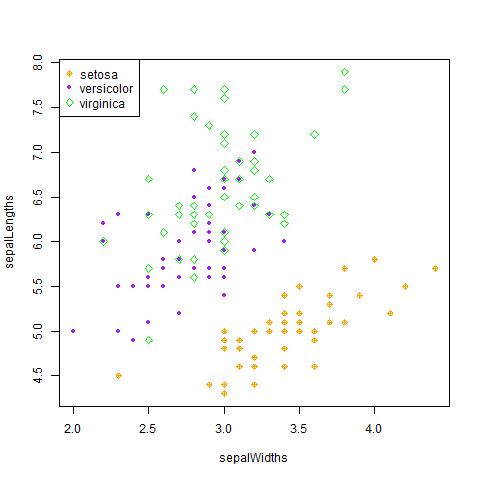
\includegraphics[width=15cm,height=15cm]{iris.png}
	\caption[petal length vs petal width]{petal length vs petal width}
	\label{irisInfo}
\end{figure}
\item Can you distinguish one species from another by just looking at the plot you created?
Observation: The orange points are clearer than the green and purple points since they do not overlap as much
\end{enumerate}

\item (20pts) A TV game show called \emph{let's Make a Deal},was popular in the 1960s and 1970s. A contestant in the show as given a choice of three doors. Behind one door was a valuable prizes. After a contestant chose a door, say Door 1, the host opened one of the other two doors, say Door 3, showing a less valuable prize. He then gave the contestant the opportunity to switch from Door 1 to Door 2. Would switching from Door 1 to Door 2 increase the contestant's chances of winning the car?
\begin{enumerate}
\item Find the theoretical probability of winning if the contestant switch the door.\\
{\color{blue} Solution: 
	\[
		P(D1)=\frac{1}{3} \rightarrow P(D2\text{ or }D3)=\frac{2}{3}
	\]
	Two things can happen here, either I chose the right door on my first guess,

	 meaning door 2 or door 3 will be opened with equal probablity, or I chose incorrectly, and the other bogus door is revealed.\\
	 In the case I chose incorrectly, switching causes me to win every time \\
	 In the case I chose correctly, switching doors causes me to lose every time.\\
	 I will choose incorrectly to begin with $\frac{2}{3}$ of the time.\\
	 If I switch all the time, my chances of winning are thus $\frac{2}{3}$, which is an improvement! 
}
\item Use software R to conduct a simulation to confirm your solution.\\
{\color{blue} Solution: Describe how did you design the simulation clearly.
\begin{verbatim}
#this is where i never switch
oDoor=sample(c(1,2,3),100,1)
results=table(oDoor)
myPick=sample(c(1,2,3),100,1)
correct = 0
for(i in 1:100){
if(oDoor[i]==myPick[i]){
correct = correct+1
#this shows the chance I got it right the first time
}
}
print(correct/100.0)
#this is when I always switch
oDoor=sample(c(1,2,3),100,1)
results=table(oDoor)
myPick=sample(c(1,2,3),100,1)
correct = 0
for(i in 1:100){
reveal=1:3
if(oDoor[i]==myPick[i]){
#i initially picked the correct door, but I am going to switch, so I dont get any correct
}
else
{
#now I pick the correct door! he revealed the other bogus door and I switch to choose the prize!
correct=correct + 1
}
}
print(correct/100.0)
\end{verbatim}
}
Hint: check out the use of R function ``sample()";
\end{enumerate}
\end{enumerate}

\end{document}
